\documentclass[12pt]{article}
\usepackage[utf8]{inputenc}
\usepackage[french]{babel}
\usepackage{amsmath,amsthm,amsfonts,amssymb}
\usepackage{lmodern}
\usepackage[top=2.4cm,bottom=2.4cm,left=2cm,right=2cm]{geometry}
\usepackage{hyperref}
\usepackage{multicol}
\usepackage{enumitem}
\usepackage{listings}
\usepackage[dvipsnames]{xcolor}
\usepackage{tikz}

%\date{}
\title{{\bf  Génie logiciel} \\
	Notes du cours de 16/12  \\
	{\small L3 Informatique appliquée 2022-2023} \\
	{\it \small MABROUK Fayez}}
\begin{document}
	\maketitle
	\newpage
	\section{Programmation}
	\section{Paradigmes de programmation}
	\subsection{Paradigmes de programmation}
	\begin{itemize}
		\item[* ] Paradigmes de programmation
		Un paradigme de programmation est un style de programmation d'un ordinateur défini par un ensemble spécifique de concepts et de techniques de programmation.
		, incarné par son langage noyau, le petit langage de base dans lequel toutes les abstractions du paradigme peuvent être définies.
		\begin{figure}[!hbtp]
			\centering
			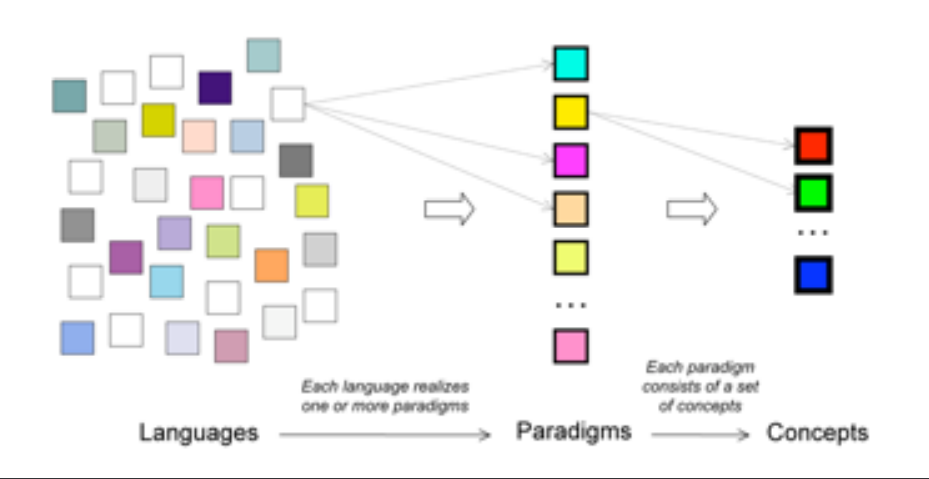
\includegraphics[scale=0.75]{Capture.PNG}
			%\caption{Légende de l'image}
		\end{figure}
	\end{itemize}
\end{document}